\chapter{Simulation methods}\label{chap5}

In the previous chapters, we focused on conjugate families, where the posterior and predictive distributions have standard analytical forms (e.g., normal, Student's t, gamma, binomial, Poisson, etc.) and where the marginal likelihood has a closed-form analytical solution. However, realistic models are often more complex and lack such closed-form solutions.

To address this complexity, we rely on simulation (stochastic) methods to draw samples from posterior and predictive distributions. This chapter introduces posterior simulation, a cornerstone of Bayesian inference. We discuss Markov Chain Monte Carlo (MCMC) methods, including Gibbs sampling, Metropolis-Hastings, and Hamiltonian Monte Carlo, as well as other techniques like importance sampling and particle filtering (sequential Monte Carlo).

The simulation methods discussed in this chapter are specifically applied throughout this book. However, we do not delve into deterministic methods, such as numerical integration (quadrature), or other simulation methods, including discrete approximation, the probability integral transform, the method of composition, accept-reject sampling, and slice sampling algorithms. While these methods are also widely used, they are not as common as the approaches explicitly employed in this book.

For readers interested in these alternative methods, we recommend exploring \cite[Chaps.~2 and 3]{robert2010introducing}, \cite[Chaps.~2, 3, and 8]{robert2011monte}, \cite[Chap.~5]{greenberg2012introduction}, and \cite[Chap.~10]{gelman2021bayesian}.

\section{Markov chain Monte Carlo methods}\label{sec51}

Markov Chain Monte Carlo (MCMC) methods are algorithms used to approximate complex probability distributions by constructing a Markov chain. This chain is a sequence of random samples where each sample depends only on the previous one. The goal of MCMC methods is to obtain draws from the posterior distribution as the equilibrium distribution. The key point in MCMC methods is the transition kernel or density, $q(\bm{\theta}^{(s)}|\bm{\theta}^{(s-1)})$, which generates a draw $\bm{\theta}^{(s)}$ at stage $s$ that depends solely on $\bm{\theta}^{(s-1)}$. This transition distribution must be designed such that the Markov chain converges to a unique stationary distribution, which, in our case, is the posterior distribution, that is, $\pi(\bm{\theta}^{(s)}|\bm{y})=\int_{\bm{\Theta}}q(\bm{\theta}^{(s)}|\bm{\theta}^{(s-1)})\pi(\bm{\theta}^{(s-1)}|\bm{y})d\bm{\theta}^{(s-1)}$.

Given that we start at an arbitrary point, $\bm{\theta}^{(0)}$, the algorithm requires that the Markov chain be \textit{irreducible}, meaning that the process can reach any other state with positive probability. Additionally, the process must be \textit{aperiodic}, meaning that for each state, the greatest common divisor of the number of steps it takes to return to the state is 1, ensuring that there are no cycles forcing the system to return to a state only after a fixed number of steps. Furthermore, the process must be \textit{recurrent}, meaning that it will return to any state an infinite number of times with probability one. However, to ensure convergence to the stationary distribution, a stronger condition is required: the process must be \textit{positive recurrent}, meaning that the expected return time to a state is finite. Given an \textit{irreducible}, \textit{aperiodic}, and \textit{positive recurrent} transition density, the Markov chain algorithm will asymptotically converge to the stationary posterior distribution we are seeking. For more details, see \cite[chap.~6]{robert2011monte}.
   

\subsection{Gibbs sampler}\label{sec511}

This Gibbs sampler algorithm is one of the most widely used MCMC methods for sampling from non-standard distributions in Bayesian analysis. While it is a special case of the Metropolis-Hastings (MH) algorithm, it originated from a different theoretical background \cite{Geman1984,Gelfand1990}. The key requirement for implementing the Gibbs sampling algorithm is the availability of conditional posterior distributions. The algorithm works by cycling through the conditional posterior distributions corresponding to different blocks of the parameter space under inference.

Two simplify concepts let's focus on a parameter space composed by two blocks, $\bm{\theta} = [\bm{\theta}_1 \ \bm{\theta}_2]^{\top}$, the Gibbs sampling algorithm uses as transition kernel $q(\bm{\theta}_1^{(s)},\bm{\theta}_2^{(s)}|\bm{\theta}_1^{(s-1)},\bm{\theta}_2^{(s-1)})=\pi(\bm{\theta}_1^{(s)}|\bm{\theta}_2^{(s-1)},\bm{y})\pi(\bm{\theta}_2^{(s)}|\bm{\theta}_1^{(s)},\bm{y})$. Thus,
{\scriptsize
\begin{align*}
	\int_{\bm{\Theta}}q(\bm{\theta}^{(s)}|\bm{\theta}^{(s-1)})\pi(\bm{\theta}^{(s-1)}|\bm{y})d\bm{\theta}^{(s-1)}
	&=\int_{\bm{\Theta}_2}\int_{\bm{\Theta}_1}\pi(\bm{\theta}_1^{(s)}|\bm{\theta}_2^{(s-1)},\bm{y})\pi(\bm{\theta}_2^{(s)}|\bm{\theta}_1^{(s)},\bm{y})\pi(\bm{\theta}^{(s-1)}_1,\bm{\theta}^{(s-1)}_2|\bm{y})d\bm{\theta}^{(s-1)}_1d\bm{\theta}^{(s-1)}_2\\
	&=\pi(\bm{\theta}_2^{(s)}|\bm{\theta}_1^{(s)},\bm{y})\int_{\bm{\Theta}_2}\int_{\bm{\Theta}_1}\pi(\bm{\theta}_1^{(s)}|\bm{\theta}_2^{(s-1)},\bm{y})\pi(\bm{\theta}^{(s-1)}_1,\bm{\theta}^{(s-1)}_2|\bm{y})d\bm{\theta}^{(s-1)}_1d\bm{\theta}^{(s-1)}_2\\
	&=\pi(\bm{\theta}_2^{(s)}|\bm{\theta}_1^{(s)},\bm{y})\int_{\bm{\Theta}_2}\pi(\bm{\theta}_1^{(s)}|\bm{\theta}_2^{(s-1)},\bm{y})\pi(\bm{\theta}^{(s-1)}_2|\bm{y})d\bm{\theta}^{(s-1)}_2\\
	&=\pi(\bm{\theta}_2^{(s)}|\bm{\theta}_1^{(s)},\bm{y})\int_{\bm{\Theta}_2}\pi(\bm{\theta}_1^{(s)},\bm{\theta}_2^{(s-1)}|\bm{y})d\bm{\theta}^{(s-1)}_2\\
	&=\pi(\bm{\theta}_2^{(s)}|\bm{\theta}_1^{(s)},\bm{y})\pi(\bm{\theta}_1^{(s)}|\bm{y})\\
	&=\pi(\bm{\theta}_1^{(s)},\bm{\theta}_2^{(s)}|\bm{y}).\\
\end{align*}
}
Then, $\pi(\bm{\theta}|\bm{y})$ is the stationary distribution for the Gibbs transition kernel.

A word of caution! Even if we have well-defined conditional posterior distributions $\pi(\bm{\theta}_1^{(s)} | \bm{\theta}_2^{(s-1)}, \bm{y})$ and $\pi(\bm{\theta}_2^{(s)} | \bm{\theta}_1^{(s)}, \bm{y})$, and we can simulate from them, the joint posterior distribution $\pi(\bm{\theta}_1^{(s)}, \bm{\theta}_2^{(s)} | \bm{y})$ may not correspond to any proper distribution. We should be mindful of this situation, especially when dealing with improper prior distributions (see \cite[Chap.~10]{robert2011monte} for details).

Algorithm \ref{Alg:Gibbs} demonstrates the implementation of a Gibbs sampler with $d$ blocks. The number of iterations ($S$) is chosen to ensure convergence to the stationary distribution. In Section \ref{sec54}, we review several convergence diagnostics to assess whether the posterior draws have reached convergence.

\begin{algorithm}[h!]
	\caption{Gibbs sampling}\label{Alg:Gibbs}
	\begin{algorithmic}[1]  		 			
		\State Set $\bm{\theta}_2^{(0)}$, $\bm{\theta}_3^{(0)}$, ..., $\bm{\theta}_d^{(0)}$
		\For{\texttt{$s=1,\dots,S$}}
		\State Draw $\bm{\theta}_1^{(s)}$ from $\pi(\bm{\theta}_1^{(s)}|\bm{\theta}_2^{(s-1)},\dots,\bm{\theta}_d^{(s-1)},\bm{y})$
		\State Draw $\bm{\theta}_2^{(s)}$ from $\pi(\bm{\theta}_2^{(s)}|\bm{\theta}_1^{(s)},\dots,\bm{\theta}_d^{(s-1)},\bm{y})$
		\State $\vdots$
		\State Draw $\bm{\theta}_d^{(s)}$ from $\pi(\bm{\theta}_d^{(s)}|\bm{\theta}_1^{(s)},\dots,\bm{\theta}_{d-1}^{(s)},\bm{y})$ 
		\EndFor 
		\end{algorithmic} 
\end{algorithm}

\textbf{Example: Mining disaster change point}

Let's use the dataset \textit{Mining.csv} provided by \cite{carlin1992hierarchical}. This dataset records the number of mining disasters per year from 1851 to 1962 in British coal mines.

We assume there is an unknown structural change point in the number of mining disasters, where the parameters of the Poisson distributions change. In particular,
\begin{align*}
	p(y_t)=\begin{Bmatrix}
		\frac{\exp(-\lambda_1)\lambda_1^{y_t}}{y_t!}, & t=1,2,\dots,H\\
		\frac{\exp(-\lambda_2)\lambda_2^{y_t}}{y_t!}, & t=H+1,\dots,T\\
	\end{Bmatrix},
\end{align*}  
where $H$ is the changing point.

We use conjugate families for $\lambda_l$, $l = 1, 2$, where $\lambda_l \sim G(\alpha_{l0}, \beta_{l0})$, and set $\pi(H) = 1 / T$, which corresponds to a discrete uniform distribution for the change point. This implies that, a priori, we assume equal probability for any time to be the change point.

The posterior distribution is
\begin{align*}
	\pi(\lambda_1,\lambda_2,H|\bm{y})&\propto \prod_{t=1}^{H} \frac{\exp(-\lambda_1)\lambda_1^{y_t}}{y_t!} \prod_{t=H+1}^{T}\frac{\exp(-\lambda_2)\lambda_2^{y_t}}{y_t!}\\
	&\times \exp(-\beta_{10}\lambda_1)\lambda_1^{\alpha_{10}-1} \exp(-\beta_{20}\lambda_2)\lambda_2^{\alpha_{20}-1} 1/T\\
	&\propto\exp(-H\lambda_1)\lambda_1^{\sum_{t=1}^H y_t}\exp(-(T-H)\lambda_2)\lambda_2^{\sum_{t=H+1}^T y_t}\\
	&\times \exp(-\beta_{10}\lambda_1)\lambda_1^{\alpha_{10}-1} \exp(-\beta_{20}\lambda_2)\lambda_2^{\alpha_{20}-1}.
\end{align*} 
Then, the conditional posterior distribution of $\lambda_1|\lambda_2,H,\bm{y}$ is 
\begin{align*}
	\pi(\lambda_1|\lambda_2,H,\bm{y})&\propto\exp(-(H+\beta_{10})\lambda_1)\lambda_1^{\sum_{t=1}^H y_t+\alpha_{10}-1},
\end{align*} 
that is, $\lambda_1|\lambda_2,H,\bm{y}\sim G(\alpha_{1n},\beta_{1n})$, $\beta_{1n}=H+\beta_{10}$ and $\alpha_{1n}=\sum_{t=1}^H y_t+\alpha_{10}$.

The conditional posterior distribution of $\lambda_2|\lambda_1,H,\bm{y}$ is 
\begin{align*}
	\pi(\lambda_2|\lambda_1,H,\bm{y})&\propto\exp(-((T-H)+\beta_{20})\lambda_2)\lambda_2^{\sum_{t=H+1}^T y_t+\alpha_{20}-1},
\end{align*} 
that is, $\lambda_2|\lambda_1,H,\bm{y}\sim G(\alpha_{2n},\beta_{2n})$, $\beta_{2n}=(T-H)+\beta_{20}$ and $\alpha_{2n}=\sum_{t=H+1}^T y_t+\alpha_{20}$.

The conditional posterior distribution of the change point is
\begin{align*}
	\pi(H|\lambda_1,\lambda_2,\bm{y})&\propto\exp(-H\lambda_1)\lambda_1^{\sum_{t=1}^H y_t}\exp(-(T-H)\lambda_2)\lambda_2^{\sum_{t=H+1}^T y_t}\\
	&\propto \exp(-H(\lambda_1-\lambda_2))\lambda_1^{\sum_{t=1}^H y_t}\lambda_2^{\sum_{t=H+1}^T y_t} \exp(-T\lambda_2) \frac{\lambda_2^{\sum_{t=1}^H}}{\lambda_2^{\sum_{t=1}^H} y_t}\\
	&\propto \exp(-H(\lambda_1-\lambda_2))\left(\frac{\lambda_1}{\lambda_2}\right)^{\sum_{t=1}^H y_t}.
\end{align*} 
Thus, the conditional posterior distribution of $H$ is
\begin{align*}
	\pi(H|\lambda_1,\lambda_2,\bm{y})=& \frac{\exp(-H(\lambda_1-\lambda_2))\left(\frac{\lambda_1}{\lambda_2}\right)^{\sum_{t=1}^H y_t}}{\sum_{H=1}^T \exp(-H(\lambda_1-\lambda_2))\left(\frac{\lambda_1}{\lambda_2}\right)^{\sum_{t=1}^H y_t}}, & H=1,2,\dots,T.
\end{align*}
The following code shows how to do a Gibbs sampling algorithm to perform inference of this model using the hyperparameters suggested by \cite[Chap.~7]{greenberg2012introduction}, $\alpha_{l0}=0.5$ and $\beta_{l0}=1$, $l=1,2$.

\begin{tcolorbox}[enhanced,width=4.67in,center upper,
	fontupper=\large\bfseries,drop shadow southwest,sharp corners]
	\textit{R code. Gibbs sampler: The mining disaster changepoint}
	\begin{VF}
		\begin{lstlisting}[language=R]
rm(list = ls()); set.seed(010101)
dataset<-read.csv("https://raw.githubusercontent.com/besmarter/BSTApp/refs/heads/master/DataApp/MiningDataCarlin.csv",header=T)
attach(dataset); str(dataset)
a10<-0.5; a20<-0.5
b10<-1; b20<-1
y<-Count
sumy<-sum(Count); N<-length(Count)
theta1<-NULL; theta2<-NULL
kk<-NULL; k<-60; S<-10000
for(i in 1:S){
	a1<-a10+sum(y[1:k]); b1<-b10+k
	theta11<-rgamma(1,a1,b1)
	theta1<-c(theta1,theta11)
	a2<-a20+sum(y[(1+k):N]); b2<-b20+N-k
	theta22<-rgamma(1,a2,b2)
	theta2<-c(theta2,theta22)
	pp<-NULL
	for(l in 1:N){
		p<-exp(l*(theta22-theta11))*(theta11/theta22)^(sum(y[1:l]))
		pp<-c(pp,p)
	}
	prob<-pp/sum(pp); k<-sample(1:N,1,prob=prob)
	kk<-c(kk,k)
}
library(coda); plot(mcmc(theta1)); summary(mcmc(theta1)); autocorr.plot(mcmc(theta1))
plot(mcmc(theta2)); summary(mcmc(theta2)); autocorr.plot(mcmc(theta2))
plot(mcmc(kk)); summary(mcmc(kk)); autocorr.plot(mcmc(kk))
\end{lstlisting}
	\end{VF}
\end{tcolorbox} 

The posterior results indicate that the rate of disasters decrease from 3.1 to 0.92 per year in 1890. 

Figure \ref{fig52} shows the histogram of the posterior draws of the change point in mining disasters. 

\begin{figure}[!h]
	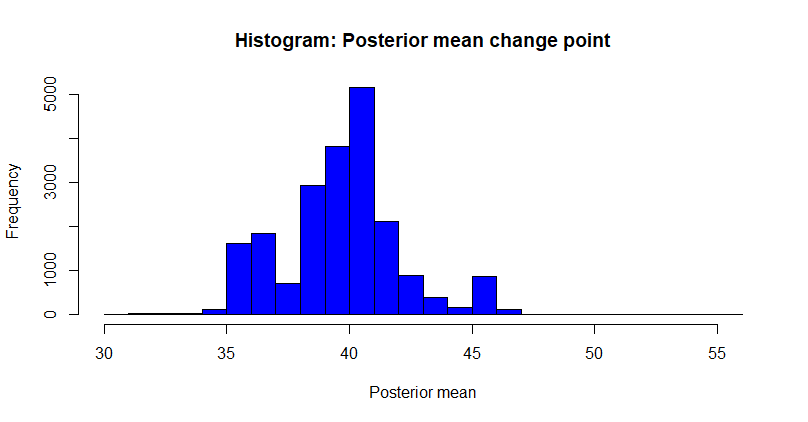
\includegraphics[width=340pt, height=200pt]{Chapters/chapter5/figures/Mining.png}
	%%\centerline{\epsfig{/Chapters/chapter1/figures/cat.eps,width=.8\textheight,height=.4\textwidth}}
	\caption[List of figure caption goes here]{Histogram of posterior draws of change point: Mining disasters}\label{fig52}
\end{figure} 

\subsection{Metropolis-Hastings}\label{sec512}

The Metropolis-Hastings (M-H) algorithm \cite{metropolis53,hastings70} is a general MCMC method that does not require standard closed-form solutions for the conditional posterior distributions. The key idea is to use a transition kernel whose unique invariant distribution is $\pi(\bm{\theta} | \bm{y})$. This kernel must satisfy the \textit{balancing condition}, meaning that, given a realization $\bm{\theta}^{(s-1)}$ at stage $s-1$ from the stationary distribution $\pi(\bm{\theta} | \bm{y})$, we generate a candidate draw $\bm{\theta}^{c}$ from the \textit{proposal distribution} $q(\bm{\theta}^{c} | \bm{\theta}^{(s-1)})$ at stage $s$ such that:
\[
q(\bm{\theta}^{c} | \bm{\theta}^{(s-1)}) \pi(\bm{\theta}^{(s-1)} | \bm{y}) = q(\bm{\theta}^{(s-1)} | \bm{\theta}^{c}) \pi(\bm{\theta}^{c} | \bm{y}),
\]

which implies that the probability of moving from $\bm{\theta}^{(s-1)}$ to $\bm{\theta}^{c}$ is equal to the probability of moving from $\bm{\theta}^{c}$ to $\bm{\theta}^{(s-1)}$.

In general, the \textit{balancing condition} is not automatically satisfied, and we must introduce an acceptance probability $\alpha(\bm{\theta}^{(s-1)}, \bm{\theta}^{c})$ to ensure that the condition holds:
\[
q(\bm{\theta}^{c} | \bm{\theta}^{(s-1)}) \pi(\bm{\theta}^{(s-1)} | \bm{y}) \alpha(\bm{\theta}^{(s-1)}, \bm{\theta}^{c}) = q(\bm{\theta}^{(s-1)} | \bm{\theta}^{c}) \pi(\bm{\theta}^{c} | \bm{y}).
\]

Thus, the acceptance probability is given by:

\[
\alpha(\bm{\theta}^{(s-1)}, \bm{\theta}^{c}) = 
\min\left\{\frac{q(\bm{\theta}^{(s-1)} | \bm{\theta}^{c}) \pi(\bm{\theta}^{c} | \bm{y})}{q(\bm{\theta}^{c} | \bm{\theta}^{(s-1)}) \pi(\bm{\theta}^{(s-1)} | \bm{y})}, 1\right\},
\]

where $q(\bm{\theta}^{c} | \bm{\theta}^{(s-1)})$ and $\pi(\bm{\theta}^{(s-1)} | \bm{y})$ must be nonzero, as transitioning from $\bm{\theta}^{(s-1)}$ to $\bm{\theta}^{c}$ is only possible under these conditions.

Algorithm \ref{Alg:MH} shows how to implement a Metropolis-Hastings algorithm.  The number of iterations ($S$) is chosen to ensure convergence to the stationary distribution. 

\begin{algorithm}[h!]
	\caption{Metropolis-Hastings algorithm}\label{Alg:MH}
	\begin{algorithmic}[1]
		\State Set $\bm{\theta}^{(0)}$ in the support of $\pi(\bm{\theta}|\bm{y})$  		 			
		\For{\texttt{$s=1,\dots,S$}}
		\State Draw $\bm{\theta}^{c}$ from $q(\bm{\theta}^{c}|\bm{\theta}^{(s-1)})$
		\State Calculate $\alpha(\bm{\theta}^{(s-1)}, \bm{\theta}^{c}) = 
		\min\left\{\frac{q(\bm{\theta}^{(s-1)} | \bm{\theta}^{c}) \pi(\bm{\theta}^{c} | \bm{y})}{q(\bm{\theta}^{c} | \bm{\theta}^{(s-1)}) \pi(\bm{\theta}^{(s-1)} | \bm{y})}, 1\right\}$
		\State Draw $U$ from $U(0,1)$
		\State $\bm{\theta}^{(s)}=\begin{Bmatrix}
			\bm{\theta}^{c} & \text{if } U\leq \alpha(\bm{\theta}^{(s-1)}, \bm{\theta}^{c})\\
			\bm{\theta}^{(s-1)} & \text{otherwise}\\
		\end{Bmatrix}$
		\EndFor 
	\end{algorithmic} 
\end{algorithm}

Some remarks: First, we do not need to know the marginal likelihood to implement the M-H algorithm, as it cancels out when calculating the acceptance probability. Specifically, given that $\pi(\bm{\theta}|\bm{y}) \propto \pi(\bm{\theta}) \times p(\bm{y}|\bm{\theta})$, we can use the right-hand side expression to compute the acceptance probability. Second, the Gibbs sampling algorithm is a particular case of the M-H algorithm where the acceptance probability is equal to 1 (\cite{Gelman1992} and \cite[Chap.~10]{robert2011monte}, see Exercise 2). Third, we can combine the M-H and Gibbs sampling algorithms when dealing with relatively complex posterior distributions. Specifically, the Gibbs sampling algorithm can be used for blocks with conditional posterior distributions in standard closed forms, while the M-H algorithm is applied to sample from conditional posterior distributions that do not have standard forms. This approach is known as the M-H within Gibbs sampling algorithm. Fourth, we can note that the transition kernel in the M-H algorithm is a mixture of a continuous density ($q(\bm{\theta}^{c} | \bm{\theta}^{(s-1)})$) and a probability mass function ($\alpha(\bm{\theta}^{(s-1)}, \bm{\theta}^{c})$) \cite{chib1995understanding}. 

Fifth, a crucial point associated with the proposal densities is the acceptance probability. Low or high acceptance probabilities are not ideal. A low rate implies poor mixing, meaning the chain does not move effectively through the support of the posterior distribution. Conversely, a high acceptance rate implies that the chain will converge too slowly. A sensible value depends on the dimension of the parameter space. A rule of thumb is that if the dimension is less than or equal to 2, the acceptance rate should be around 0.50. If the dimension is greater than 2, the acceptance rate should be approximately 0.25 \cite{Roberts1997}. For technical details of the Metropolis-Hastings algorithm, see \cite[Chap.~7]{robert2011monte}.

Regarding the proposal density, it must be positive everywhere the posterior distribution is positive. This ensures that the Markov chain can explore the entire support of the posterior distribution. Additionally, the proposal density must allow the Markov chain to reach any region of the posterior distribution's support. There are three standard approaches for choosing the proposal density: the independent proposal, the random walk proposal, and the tailored proposal.

In the independent proposal, $q(\bm{\theta}^{c} | \bm{\theta}^{(s-1)}) = q(\bm{\theta}^{c})$, which implies that 

\[
\alpha(\bm{\theta}^{(s-1)}, \bm{\theta}^{c}) = 
\min\left\{\frac{q(\bm{\theta}^{(s-1)}) \pi(\bm{\theta}^{c} | \bm{y})}{q(\bm{\theta}^{c}) \pi(\bm{\theta}^{(s-1)} | \bm{y})}, 1\right\}.
\]

In this case, a move from $\bm{\theta}^{(s-1)}$ to $\bm{\theta}^{c}$ is always accepted if $q(\bm{\theta}^{(s-1)}) \pi(\bm{\theta}^{c} | \bm{y}) \geq q(\bm{\theta}^{c}) \pi(\bm{\theta}^{(s-1)} | \bm{y})$.

In the random walk proposal, $\bm{\theta}^{c} = \bm{\theta}^{(s-1)} + \bm{\epsilon}$, where $\bm{\epsilon}$ is a random perturbation. If $p(\bm{\epsilon}) = p(-\bm{\epsilon})$, meaning the distribution of $p(\bm{\epsilon})$ is symmetric around zero, then $q(\bm{\theta}^{c} | \bm{\theta}^{(s-1)}) = q(\bm{\theta}^{(s-1)} | \bm{\theta}^{c})$. This was the original Metropolis algorithm \cite{metropolis53}. Thus, the acceptance rate is 

\[
\alpha(\bm{\theta}^{(s-1)}, \bm{\theta}^{c}) = 
\min\left\{\frac{\pi(\bm{\theta}^{c} | \bm{y})}{\pi(\bm{\theta}^{(s-1)} | \bm{y})}, 1\right\}.
\]

In this case, a move from $\bm{\theta}^{(s-1)}$ to $\bm{\theta}^{c}$ is always accepted if $\pi(\bm{\theta}^{c} | \bm{y}) \geq \pi(\bm{\theta}^{(s-1)} | \bm{y})$.

In the tailored proposal, the density is designed to have fat tails, is centered at the mode of the posterior distribution, and its scale matrix is given by the negative inverse Hessian matrix evaluated at the mode. Specifically, for two blocks, the log posterior distribution is maximized with respect to $\bm{\theta}_1$ given $\bm{\theta}_2$. This process is repeated at each iteration of the algorithm because $\bm{\theta}_2$ changes at different stages. As a result, the algorithm can be slow since the optimization process is computationally demanding (see \cite[Chap.~7 and 9]{greenberg2012introduction} for examples).

A sensible recommendation when performing M-H algorithm is to use a random walk proposal such that $\bm{\epsilon}\sim N(\bm{0},c^2\bm{\Sigma})$, where $\bm{\Sigma}$ is the negative inverse Hessian matrix evaluated at the mode, that is, maximize with respect to all parameters, and set $c\approx 2.4/\sqrt{dim\left\{\bm{\theta}\right\}}$, which is the most efficient scale compared to independent sampling \cite[Chap.~12]{gelman2021bayesian}. After some iterations of the algorithm, adjust the scale matrix $\bm{\Sigma}$ as before, and increase or decrease $c$ if the acceptance rate of the simulations is too high or low, respectively. The objective is to bring the acceptance rate to the stated rule of thumb, that is, if the dimension is less than or equal to 2, the acceptance rate should be around 0.50, and if the dimension is greater than 2, the acceptance rate should be around 0.25. Once this is achieved, we should run the algorithm without modifications and use this part of the algorithm to perform inference.\\


\textbf{Example: Ph.D. students sleeping hours continues}

In the Ph.D. students sleeping hours exercise of Chapter \ref{chap4} we get a posterior distribution that is Beta with parameters 16.55 and 39.57. We can sample from this posterior distribution using the function \textit{rbeta} from \textbf{R}. However, we want to compare the performance of a M-H algorithm using as proposal density a $U(0,1)$ distribution.

The following code shows how to do a M-H algorithm to sample from the beta distribution using the uniform distribution.

\begin{tcolorbox}[enhanced,width=4.67in,center upper,
	fontupper=\large\bfseries,drop shadow southwest,sharp corners]
	\textit{R code. Metropolis-Hastings algorithm:  Ph.D. students sleeping hours}
	\begin{VF}
		\begin{lstlisting}[language=R]
rm(list = ls()); set.seed(010101)
an <- 16.55; bn <- 39.57
S <- 100000; p <- runif(S); accept <- rep(0, S)
for (s in 2:S){
	pc <- runif(1) # Candidate
	a <- dbeta(pc, an, bn)/dbeta(p[s-1], an, bn) # Acceptance rate
	U <- runif(1)
	if(U <= a){
		p[s] <- pc
		accept[s] <- 1
	}else{
		p[s] <- p[s-1]
		accept[s] <- 0
	}
}
mean(accept); mean(p); sd(p)
an/(an + bn); (an*bn/((an+bn)^2*(an+bn+1)))^0.5 # Population values
h <- hist(p, breaks=50, col="blue", xlab="Proportion Ph.D. students sleeping at least 6 hours", main="Beta draws from a Metropolis-Hastings algorithm")
pfit <- seq(min(p),max(p),length=50)
yfit<-dbeta(pfit, an, bn)
yfit <- yfit*diff(h$mids[1:2])*length(p)
lines(pfit, yfit, col="red", lwd=2)
\end{lstlisting}
	\end{VF}
\end{tcolorbox} 

The results indicate that the mean and standard deviation obtained from the posterior draws are similar to the population values. Furthermore, Figure \ref{fig53} presents the histogram of the posterior draws alongside the density of the beta distribution, demonstrating a good match between them.

\begin{figure}[!h]
	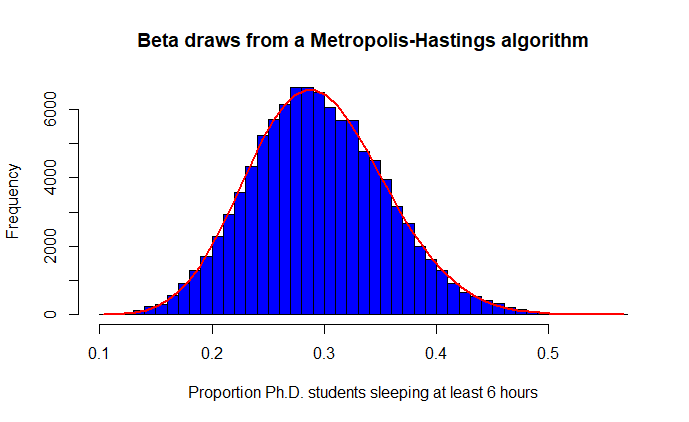
\includegraphics[width=340pt, height=200pt]{Chapters/chapter5/figures/Beta.png}
	%%\centerline{\epsfig{/Chapters/chapter1/figures/cat.eps,width=.8\textheight,height=.4\textwidth}}
	\caption[List of figure caption goes here]{Histogram of posterior draws of beta distribution and the density of the beta distribution.}\label{fig53}
\end{figure}      

\subsection{Hamiltonian Monte Carlo}\label{sec523}

Hamiltonian Monte Carlo (HMC) was proposed by \cite{duane1987hybrid} and later introduced to the statistical community by \cite{neal1996bayesian}. HMC extends the Metropolis algorithm to efficiently explore the parameter space by introducing \textit{momentum variables}, which help overcome the random walk behavior of Gibbs sampling and the Metropolis-Hastings algorithm. Known also as hybrid Monte Carlo, HMC is particularly advantageous for high-dimensional posterior distributions, as it reduces the risk of getting stuck in local modes and significantly improves mixing \cite{neal2011mcmc}. 

However, HMC is designed to work with strictly positive target densities. Therefore, transformations are required to handle bounded parameters, such as variances and proportions. For example, logarithmic and logit transformations can be applied. These transformations necessitate the use of the change-of-variable theorem to compute the log posterior density and its gradient, which are essential for implementing the HMC algorithm.

HMC leverages concepts from physics, specifically Hamiltonian mechanics, to propose transitions in the Markov chain. In Hamiltonian mechanics, two key variables define the total energy of the system: the \textit{position} (\(\bm{\theta}\)) and the \textit{momentum} (\(\bm{\delta}\)). The Hamiltonian represents the total energy of the system, consisting of \textit{potential energy} (energy due to position) and \textit{kinetic energy} (energy associated with motion). The objective is to identify trajectories that preserve the system's total energy, meaning the Hamiltonian remains invariant, while avoiding trajectories that do not. This approach enhances the acceptance rate of proposed transitions.

To implement HMC, we solve the differential equations derived from the Hamiltonian, which involve derivatives with respect to position and momentum. However, these equations rarely have analytical solutions, requiring numerical methods for approximation. This necessitates discretizing Hamilton’s equations, which introduces errors. To mitigate these errors, HMC uses the \textit{leapfrog integrator}, a numerical method with smaller errors compared to simpler approaches like the Euler method.

HMC uses a \textit{momentum variable} (\(\delta_k\)) for each \(\theta_k\), so that the transition kernel of \(\bm{\theta}\) is determined by \(\bm{\delta}\). Both vectors are updated using a Metropolis algorithm at each stage such that the distribution of \(\bm{\theta}\) remains invariant \cite{neal2011mcmc}. The joint density in HMC is given by \( p(\bm{\theta}, \bm{\delta} | \bm{y}) = \pi(\bm{\theta} | \bm{y}) \times p(\bm{\delta}) \), where \(\bm{\delta} \sim N(\bm{0}, \bm{M})\), and \(\bm{M}\) is a diagonal matrix such that \(\delta_k \sim N(0, M_{kk})\). 

Algorithm \ref{Alg:HMC} outlines the HMC implementation. The gradient vector \(\frac{d\log(\pi(\bm{\theta}|\bm{y}))}{d\bm{\theta}}\) must be computed analytically, as using finite differences can be computationally expensive. However, it is advisable to verify the analytical calculations by evaluating the gradient at the maximum posterior estimate, where the function should return values close to 0, or by comparing results with finite differences at a few points. 

\begin{algorithm}[h!]
	\caption{Hamiltonian Monte Carlo}\label{Alg:HMC}
	\begin{algorithmic}[1]
		\State Initiate at $\bm{\theta}^{(0)}$ in the support of $\pi(\bm{\theta}|\bm{y})$, and set step size $\epsilon$, number of leapfrog steps $L$, and total iterations $S$ 
		\State Draw $\bm{\delta}^{(0)}$ from $N(\bm{0}, \bm{M})$  		 			
		\For{\texttt{$s=1,\dots,S$}}
			\For{\texttt{$l=1,\dots,L$}}
				\If{l = 1}
					\State $\bm{\delta}^{c} \leftarrow \bm{\delta}^{(s-1)} + \frac{1}{2}\epsilon \frac{d\log(\pi(\bm{\theta}|\bm{y}))}{d\bm{\theta}}$
					\State $\bm{\theta}^c\leftarrow \bm{\theta}^{(s-1)}+\epsilon \bm{M}^{-1}\bm{\delta}^{c}$
				\Else
					\If{l=2,\dots,L-1}
						\State $\bm{\delta}^{c} \leftarrow \bm{\delta}^{c} + \epsilon \frac{d\log(\pi(\bm{\theta}|\bm{y}))}{d\bm{\theta}}$
						\State $\bm{\theta}^c\leftarrow \bm{\theta}^c+\epsilon \bm{M}^{-1}\bm{\delta}^{c}$
					\Else
					 	\State $\bm{\delta}^{c} \leftarrow \bm{\delta}^{c} + \frac{1}{2}\epsilon \frac{d\log(\pi(\bm{\theta}|\bm{y}))}{d\bm{\theta}}$
					 	\State $\bm{\theta}^c\leftarrow \bm{\theta}^{c}+\epsilon \bm{M}^{-1}\bm{\delta}^{c}$
					\EndIf
				\EndIf
			\EndFor
		\State Calculate $\alpha([\bm{\theta} \ \bm{\delta}]^{(s-1)}, [\bm{\theta} \ \bm{\delta}]^{c}) = 
		\min\left\{\frac{p(\bm{\delta}^{c}) \pi(\bm{\theta}^{c} | \bm{y})}{p(\bm{\delta}^{(s-1)}) \pi(\bm{\theta}^{(s-1)} | \bm{y})}, 1\right\}$
		\State Draw $U$ from $U(0,1)$
		\State $\bm{\theta}^{(s)}=\begin{Bmatrix}
			\bm{\theta}^{c} & \text{if } U\leq \alpha(\cdot, \cdot)\\
			\bm{\theta}^{(s-1)} & \text{otherwise}\\
		\end{Bmatrix}$
		\EndFor 
	\end{algorithmic} 
\end{algorithm}

Note that HMC does not require the marginal likelihood, as neither the gradient vector \(\frac{d\log(\pi(\bm{\theta}|\bm{y}))}{d\bm{\theta}}\) nor the acceptance rate depend on it. That is, we can use only \(\pi(\bm{\theta})\times p(\bm{y}|\bm{\theta})\) to implement HMC. In addition, we do not retain \(\bm{\delta}\) after it is updated at the beginning of each iteration, as it is not required subsequently. To begin, the step size (\(\epsilon\)) can be drawn randomly from a uniform distribution between 0 and \(2\epsilon_0\), and the number of leapfrog steps (\(L\)) is set as the largest integer near \(1/\epsilon\), ensuring \(\epsilon \times L \approx 1\). We need to set \(\bm{M}\) to be the inverse of the posterior covariance matrix evaluated at the maximum a posteriori estimate under this setting. 

The acceptance rate should be checked, with the optimal rate around 65\% \cite[Chap.~12]{gelman2021bayesian}. If the acceptance rate is much higher than 65\%, increase \(\epsilon_0\); if it is much lower, decrease it. This strategy may not always work, and alternative strategies can be tested, such as setting \(\bm{M} = \bm{I}\) and fine-tuning \(\epsilon\) and \(L\) to achieve an acceptance rate near 65\%. Finally, the number of iterations (\(S\)) is chosen to ensure convergence to the stationary distribution.\\

\textbf{Example: Sampling from a bi-variate Gaussian distribution}

As a toy example, let's compare the Gibbs sampling, M-H and HMC algorithms when the posterior distribuion is a bi-variate Gaussian distribution with mean $\bm{0}$ and covariance matrix $\bm{\Sigma}=\begin{bmatrix}
	1 & \rho \\
	\rho & 1
\end{bmatrix}$. Let's set $\rho= 0.98$.

The Gibbs sampler requires the conditional posterior distributions, which in this case are $\theta_1|\theta_2\sim N(\rho\theta_2,1-\rho^2)$ and $\theta_2|\theta_1\sim N(\rho\theta_1,1-\rho^2)$. We use the random walk proposal distribution for the M-H algorithm, where $\bm{\theta}^c\sim N(\bm{\theta}^{(s-1)}, \text{diag}\left\{0.18^2\right\})$. We set $\epsilon=0.05$, $L=20$ and $\bm{M}=\bm{I}_2$ for the HMC algorithm, and given that $\pi(\bm{\theta}|\bm{y})\propto \exp\left\{-\frac{1}{2}\bm{\theta}^{\top}\bm{\Sigma}^{-1}\bm{\theta}\right\}$, then $\frac{d\log(\pi(\bm{\theta}|\bm{y}))}{d\bm{\theta}}=-\bm{\Sigma}^{-1}\bm{\theta}$.

The following code shows how to implement the Gibbs sampler, the random walk M-H algorithm, and the HMC in this example such that the effective number of posterior draws is 400.

\begin{tcolorbox}[enhanced,width=4.67in,center upper,
	fontupper=\large\bfseries,drop shadow southwest,sharp corners]
	\textit{R code. Gibbs, M-H and HMC: Bi-variate normal distribution}
	\begin{VF}
		\begin{lstlisting}[language=R]
rm(list = ls()); set.seed(010101)
# Gibbs sampler
Gibbs <- function(theta, rho){
	thetal <- rnorm(1, mean = rho*theta, sd = (1- rho^2)^0.5)
	return(thetal)
}
# Metropolis-Hastings
MH <- function(theta, rho, sig2){
	SIGMA <- matrix(c(1, rho, rho, 1), 2, 2)
	SIGMAc <- matrix(c(1, sig2, sig2, 1), 2, 2)
	thetac <- MASS::mvrnorm(1, mu = theta, Sigma = SIGMAc)
	a <- mvtnorm::dmvnorm(thetac, c(0, 0), SIGMA)/mvtnorm::dmvnorm(theta, c(0, 0), SIGMA)
	U <- runif(1)
	if(U <= a){
		theta <- thetac
		accept <- 1
	}else{
		theta <- theta
		accept <- 0
	}
	return(list(theta = theta, accept = accept))
}
# Hamiltonian Monte Carlo
HMC <- function(theta, rho, epsilon, M){
	SIGMA <- matrix(c(1, rho, rho, 1), 2, 2) 
	L <- ceiling(1/epsilon)
	Minv <- solve(M); thetat <- theta
	K <- length(thetat)
	mom <- t(mvtnorm::rmvnorm(1, rep(0, K), M))
	logPost_Mom_t <- mvtnorm::dmvnorm(t(theta), rep(0, K), SIGMA, log = TRUE) +  mvtnorm::dmvnorm(t(mom), rep(0, K), M, log = TRUE)  
	for(l in 1:L){
		if(l == 1 | l == L){
			mom <- mom + 0.5*epsilon*(-solve(SIGMA)%*%theta)
			theta <- theta + epsilon*Minv%*%mom
		}else{
			mom <- mom + epsilon*(-solve(SIGMA)%*%theta)
			theta <- theta + epsilon*Minv%*%mom
		}
	}
	logPost_Mom_star <- mvtnorm::dmvnorm(t(theta), rep(0, K), SIGMA, log = TRUE) +  mvtnorm::dmvnorm(t(mom), rep(0, K), M, log = TRUE)  
	alpha <- min(1, exp(logPost_Mom_star-logPost_Mom_t))
	u <- runif(1)
	if(u <= alpha){
		thetaNew <- c(theta)
	}else{
		thetaNew <- thetat
	}
	rest <- list(theta = thetaNew, Prob = alpha)
	return(rest)
}
\end{lstlisting}
	\end{VF}
\end{tcolorbox} 


\begin{tcolorbox}[enhanced,width=4.67in,center upper,
	fontupper=\large\bfseries,drop shadow southwest,sharp corners]
	\textit{R code. Gibbs, M-H and HMC: Bi-variate normal distribution}
	\begin{VF}
		\begin{lstlisting}[language=R]
# Hyperparameters
rho <- 0.98; sig2 <- 0.18^2
# Posterior draws Gibbs and M-H
S <- 8000; thin <- 20; K <- 2
thetaPostGibbs <- matrix(NA, S, K)
thetaPostMH <- matrix(NA, S, K)
AcceptMH <- rep(NA, S)
thetaGibbs <- c(-2, 3); thetaMH <- c(-2, 3)
for(s in 1:S){
	theta1 <- Gibbs(thetaGibbs[2], rho)
	theta2 <- Gibbs(theta1, rho)
	thetaGibbs <- c(theta1, theta2)
	ResMH <- MH(thetaMH, rho, sig2)
	thetaMH <- ResMH$theta
	thetaPostGibbs[s,] <- thetaGibbs
	thetaPostMH[s,] <- thetaMH
	AcceptMH[s] <- ResMH$accept
}
keep <- seq(0, S, thin)
mean(AcceptMH[keep[-1]])
thetaPostGibbsMCMC <- coda::mcmc(thetaPostGibbs[keep[-1],])
summary(thetaPostGibbsMCMC)
coda::autocorr.plot(thetaPostGibbsMCMC)
thetaPostMHMCMC <- coda::mcmc(thetaPostMH[keep[-1],])
plot(thetaPostMHMCMC)
coda::autocorr.plot(thetaPostMHMCMC)
# Posterior draws HMC
S <- 400;epsilon <- 0.05;  L <- ceiling(1/epsilon); M <- diag(2)
thetaPostHMC <- matrix(NA, S, K)
ProbAcceptHMC  <- rep(NA, S)
thetaHMC <- c(-2, 3)
for(s in 1:S){
	ResHMC <- HMC(theta = thetaHMC, rho, epsilon, M)
	thetaHMC <- ResHMC$theta
	thetaPostHMC[s,] <- thetaHMC
	ProbAcceptHMC[s] <- ResHMC$Prob
}
thetaPostHMCMCMC <- coda::mcmc(thetaPostHMC)
plot(thetaPostHMCMCMC); coda::autocorr.plot(thetaPostHMCMCMC)
summary(ProbAcceptHMC)
#Figure
df <- as.data.frame(cbind(1:S, thetaPostHMC[,1], thetaPostMH[keep[-1],1], thetaPostGibbs[keep[-1],1]))
colnames(df) <- c("Iter", "HMC", "MH", "Gibbs")
library(latex2exp); library(ggpubr)
g1 <- ggplot(df, aes(x= Iter)) + geom_point(aes(y=HMC), colour="black") + labs(x = "Iteration", y = TeX("$\\theta_{1}$"), title = "HMC algorithm")
g2 <- ggplot(df, aes(x= Iter)) + geom_point(aes(y=MH), colour="black") + labs(x = "Iteration", y = TeX("$\\theta_{1}$"), title = "M-H algorithm")
g3 <- ggplot(df, aes(x= Iter)) + geom_point(aes(y=Gibbs), colour="black") + labs(x = "Iteration", y = TeX("$\\theta_{1}$"), title = "Gibbs sampling")
ggarrange(g3, g2, g1, labels = c("A", "B", "C"), ncol = 3, nrow = 1)
\end{lstlisting}
	\end{VF}
\end{tcolorbox} 

Figure \ref{fig54} shows the posterior draws of $\theta_1$ using the Gibbs sampler (Panel A, left), the Metropolis-Hastings algorithm (Panel B, middle), and the Hamiltonian Monte Carlo (Panel C, right). The convergence diagnostic plots (no shown) suggests that the three algorithms perform a good job. Although, the acceptance rate in HMC is higher than the M-H due to the HMC producing larger changes in $\bm{\theta}$ than a corresponding number of random-walk M-H iterations \cite{neal2011mcmc}.

\begin{figure}[!h]
	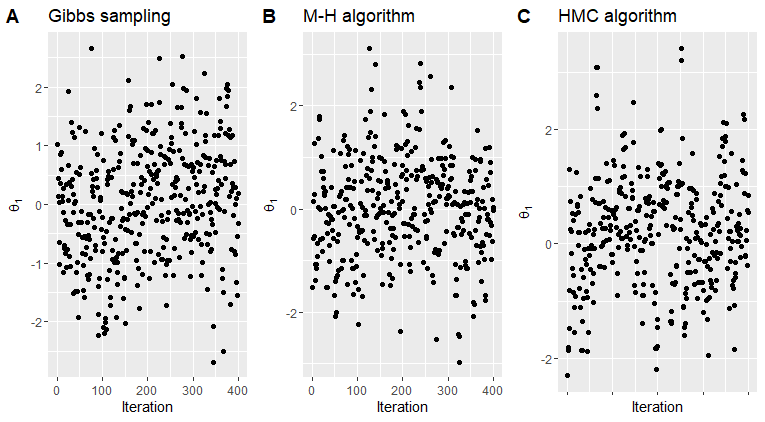
\includegraphics[width=340pt, height=200pt]{Chapters/chapter5/figures/BivariateNormal.98}
	%%\centerline{\epsfig{/Chapters/chapter1/figures/cat.eps,width=.8\textheight,height=.4\textwidth}}
	\caption[List of figure caption goes here]{Posterior draws: Gibbs sampler (A), Metropolis-Hastings (B) and Hamiltonian Monte Carlo (C) in the bivariate normal example, $\rho=0.98$.}\label{fig54}
\end{figure}       

\section{Importance sampling}\label{sec52}

Up to this section, we have introduced MCMC methods for sampling from the posterior distribution when it does not have a standard closed form. However, MCMC methods have some limitations. First, the samples are generated sequentially, which complicates parallel computing. Although multiple MCMC chains can be run simultaneously, this approach—often referred to as brute-force parallelization—does not fully address the sequential nature of individual chains. Second, consecutive samples are correlated, which reduces the effective sample size and complicates convergence diagnostics.

Thus, in this section, we introduce \textit{importance sampling} (IS), a simulation method for drawing samples from the posterior distribution that avoids these limitations. Unlike MCMC, IS does not require satisfying the balancing condition, making it conceptually and mathematically simpler to implement in certain situations. Moreover, importance weights can be reused to analyze posterior quantities, compute marginal likelihoods, compare models, approximate new target distributions, and allow for straightforward parallelization in large-scale problems.

However, the critical challenge in IS lies in selecting an appropriate proposal distribution. This involves satisfying both support and stability conditions, which can be difficult to achieve, particularly in high-dimensional problems. In such cases, MCMC methods may be more suitable.

The starting point is evaluating the integral:
\begin{align}\label{eq5_1}
	\mathbb{E}_{\pi}[h(\bm{\theta})]=\int_{\bm{\Theta}} h(\bm{\theta}) \pi(\bm{\theta}|\bm{y})d\bm{\theta},
\end{align}
where $\mathbb{E}_{\pi}$ denotes expected value under the posterior distribution.
Thus, we can approximate Equation \ref{eq5_1} by
\begin{align}\label{eq5_2}
	\bar{h}(\bm{\theta})_S=\frac{1}{S}\sum_{s=1}^S h(\bm{\theta}^{(s)}), 
\end{align}
where $\bm{\theta}^{(s)}$ are draws from $\pi(\bm{\theta}|\bm{y})$. The \textit{strong law of large numbers} shows that $\bar{h}(\bm{\theta})_S$ converges (almost surely) to $\mathbb{E}{\pi}[h(\bm{\theta})]$ as $S \rightarrow \infty$.

The challenge arises when we do not know how to obtain samples from $\pi(\bm{\theta}|\bm{y})$. The ingenious idea is to express Equation~\ref{eq5_1} in a different way using the \textit{importance sampling fundamental identity} \cite[Chap.~3]{robert2011monte}:
\begin{align}\label{eq5_3}
	\mathbb{E}_{\pi}[h(\bm{\theta})]&=\int_{\bm{\Theta}} h(\bm{\theta}) \pi(\bm{\theta}|\bm{y})\frac{q(\bm{\theta})}{q(\bm{\theta})}d\bm{\theta}\nonumber\\
	&=\mathbb{E}_{q}\left[\frac{h(\bm{\theta})\pi(\bm{\theta}|\bm{y})}{q(\bm{\theta})}\right],
\end{align}   
where $q(\bm{\theta})$ is the proposal distribution.

Thus, we have $$\frac{1}{S}\sum_{s=1}^S \left[\frac{h(\bm{\theta}^{(s)})\pi(\bm{\theta}^{(s)}|\bm{y})}{q(\bm{\theta}^{(s)})}\right]= \frac{1}{S}\sum_{s=1}^S h(\bm{\theta}^{(s)})w(\bm{\theta}^{(s)}),$$ where $w(\bm{\theta}^{(s)})= \left[\frac{\pi(\bm{\theta}^{(s)}|\bm{y})}{q(\bm{\theta}^{(s)})}\right]$ are called the \textit{importance weights}, and $\bm{\theta}^{(s)}$ are samples from the proposal distribution. This expression converges to $\mathbb{E}_{\pi}[h(\bm{\theta})]$ given that the support of $q(\bm{\theta})$ includes the support of $\pi(\bm{\theta}^{(s)}|\bm{y})$.

There are many proposal distributions that satisfy the support condition. However, the stability of the method depends heavily on the variability of the importance weights. In particular, the variance of  
\[
\frac{1}{S}\sum_{s=1}^S h(\bm{\theta}^{(s)})w(\bm{\theta}^{(s)})
\]  
can be large if the proposal distribution has lighter tails than the posterior distribution. In this case, the weights \( w(\bm{\theta}^{(s)}) \) will vary widely, assigning too much importance to a few values of \( \bm{\theta}^{(s)} \). Thus, it is important to use proposals that have thicker tails than the posterior distribution. In any case, we should check the adequacy of the proposal distribution by analyzing the behavior of the importance weights. If they are distributed more or less uniformly over the support, it is a good sign. Consider, for instance, the extreme case where $q(\bm{\theta}) = \pi(\bm{\theta}|\bm{y})$, then $w(\bm{\theta}^{(s)}) = 1$ everywhere. 

A natural choice in Bayesian inference is to use the prior distribution as the proposal, given that it is a proper density function. The prior distribution typically has heavier tails than the posterior by construction, and it is usually a distribution that allows for easy sampling.

The most relevant point for us is that importance sampling provides a way to simulate from the posterior distribution when there is no closed-form solution. The method generates samples $\bm{\theta}^{(s)}$ from $q(\bm{\theta})$ and computes the importance weights $w(\bm{\theta}^{(s)})$. Thus, if we \textit{resample} with replacement from $\bm{\theta}^{(1)},\bm{\theta}^{(2)},\dots,\bm{\theta}^{(S)}$, selecting $\bm{\theta}^{(s)}$ with probability proportional to  $w(\bm{\theta}^{(s)})$, we would get a sample $\bm{\theta}^{*(1)},\bm{\theta}^{*(2)},\dots,\bm{\theta}^{*(L)}$ of size $L$ from $\pi(\bm{\theta}|\bm{y})$ \cite{smith1992bayesian,rubin1988sir}. This is named \textit{sampling/importance resampling} (SIR) algorithm. Observe that the number of times $L^{(s)}$ each particular point $\bm{\theta}^{(s)}$ is selected follows a binomial distribution with size $L$, and probabilities proportional to $w^{(s)}$. Consequently, the vector $L_{\bm{\theta}} = \left\{L_{\bm{\theta}^1}, L_{\bm{\theta}^2}, \dots, L_{\bm{\theta}^S}\right\}$ follows a multinomial distribution with $L$ trials and probabilities proportional to $w(\bm{\theta}^{(s)})$, $s = 1, 2, \dots, S$ \cite{cappe2007overview}. Therefore, the resampling step ensures that points in the first-stage sample with small importance weights are more likely to be discarded, while points with high weights are replicated in proportion to their importance weights. In most applications, it is typical to have $S \gg L$.

The intuition is that importance weights are scaling factors that correct for the bias introduced by drawing from $q(\bm{\theta}^{(s)})$ instead of $\pi(\bm{\theta}^{(s)}|\bm{y})$; thus, when combined, the samples and weights effectively recreate the posterior distribution, ensuring the resampled data set reflects the posterior. Let's proof this 
\begin{align*}
	P(\bm{\theta}^*\in A)
	&=\frac{1}{S}\sum_{s=1}^S{w}^{(s)}\mathbbm{1}_{A}(\bm{\theta}^{(s)})\\
	&\rightarrow \mathbb{E}_q\left[\mathbbm{1}_{\in A}(\bm{\theta})\frac{\pi(\bm{\theta}|\bm{y})}{q(\bm{\theta})}\right]\\
	&=\int_{A}\left[\frac{\pi(\bm{\theta}|\bm{y})}{q(\bm{\theta})}\right]q(\bm{\theta})d\bm{\theta}\\
	&=\int_{A}\pi(\bm{\theta}|\bm{y})d\bm{\theta}. 
\end{align*}
Thus, $\bm{\theta}^*$ is approximately distributed as an observation from $\pi(\bm{\theta}|\bm{y})$.   


However, the weights $\pi(\bm{\theta}^{(s)}|\bm{y})/(Sq(\bm{\theta}^{(s)}))$ do not sum up to 1, and we need to standardize them, 
$$w^*(\bm{\theta}^{(s)})=\frac{\frac{1}{S} w(\bm{\theta}^{(s)})}{\frac{1}{S}\sum_{s=1}^Sw(\bm{\theta}^{(s)})}.$$
Note that we could alternatively arrive to these weights as follow 
\begin{align*}\label{eq5_4}
	\mathbb{E}_{\pi}[h(\bm{\theta})]&=\int_{\bm{\Theta}} \left[\frac{h(\bm{\theta}) \pi(\bm{\theta}|\bm{y})}{q(\bm{\theta})}\right]q(\bm{\theta})d\bm{\theta}\\
	&=\frac{\int_{\bm{\Theta}}\left[\frac{h(\bm{\theta}) \pi(\bm{\theta}|\bm{y})}{q(\bm{\theta})}\right] q(\bm{\theta})d\bm{\theta}}{\int_{\bm{\Theta}}\left[\frac{ \pi(\bm{\theta}|\bm{y})}{q(\bm{\theta})}\right] q(\bm{\theta})d\bm{\theta}}.
\end{align*}
Then, $$\frac{\frac{1}{S}\sum_{s=1}^Sh(\bm{\theta}^{(s)})w(\bm{\theta}^{(s)})}{\frac{1}{S}\sum_{s=1}^Sw(\bm{\theta})^{(s)}}= \sum_{s=1}^S h(\bm{\theta}^{(s)})w^*(\bm{\theta}^{(s)}).$$ This alternative expression also converges (almost surely) to $\mathbb{E}_{\pi}[h(\bm{\theta})]$.  In addition, this expression is very useful because if we do not have the marginal likelihood in the posterior distribution, this constant cancels out in $w^*(\bm{\theta}^{(s)})$. And, although this estimator is biased, the bias is small, and provides good gains in variance reduction compared with the non-standardized option \cite[Chap.~3]{robert2011monte}.

A nice by-product of implementing IS is that it easily allows the calculation of the marginal likelihood. In particular, we know from Bayes' rule that
$$p(\bm{y})^{-1}=\frac{\pi(\bm{\theta}|\bm{y})}{p(\bm{y}|\bm{\theta})\times \pi(\bm{\theta})},$$
then, 
\begin{align*}
	\int_{\bm{\Theta}}p(\bm{y})^{-1}q(\bm{\theta})d\bm{\theta}&=\int_{{\Theta}}\frac{q(\bm{\theta})}{p(\bm{y}|\bm{\theta})\times \pi(\bm{\theta})}\pi(\bm{\theta}|\bm{y})d\bm{\theta}\\
	&=\mathbb{E}_{\pi}\left[\frac{q(\bm{\theta})}{p(\bm{y}|\bm{\theta})\times \pi(\bm{\theta})}\right].
\end{align*}
Thus, an estimate of the marginal likelihood is $\left[\frac{1}{S}\sum_{s=1}^S\frac{q(\bm{\theta}^{*(s)})}{p(\bm{y}|\bm{\theta}^{*(s)})\times\pi(\bm{\theta}^{*(s)})}\right]^{-1}$. This is the Gelfand-Dey method to calculate the marginal likelihood \cite{gelfand1994bayesian} (see subsection \ref{sec10_4_3}).\\

\textbf{Example: Cauchy distribution}

Let's assume that the posterior distribution is Cauchy with parameters 0 and 1. We perform an importance sampling algorithm using as proposals a standard normal distribution and a Student's t distribution with 3 degrees of freedom. The following code shows how to do this.

\begin{tcolorbox}[enhanced,width=4.67in,center upper,
	fontupper=\large\bfseries,drop shadow southwest,sharp corners]
	\textit{R code. Importance sampling: Cauchy distribution}
	\begin{VF}
		\begin{lstlisting}[language=R]
rm(list = ls()); set.seed(010101)
S <- 20000 # Size proposal
# Importance sampling from standard normal proposal 
thetaNs <- rnorm(S)
wNs <- dcauchy(thetaNs)/dnorm(thetaNs)
wNstars <- wNs/sum(wNs)
L <- 10000 # Size posterior
thetaCauchyN <- sample(thetaNs, L, replace = TRUE, prob = wNstars)
h <- hist(thetaCauchyN, breaks=50, col="blue", xlab="x", main="Cauchy draws from importance sampling: Normal standard proposal")
pfit <- seq(min(thetaCauchyN),max(thetaCauchyN),length=50)
yfit<-dcauchy(pfit)
yfit <- yfit*diff(h$mids[1:2])*length(thetaCauchyN)
lines(pfit, yfit, col="red", lwd=2)
# Importance sampling from Student's t proposal 
df <- 3
thetaTs <- rt(S, df = df)
wTs <- dcauchy(thetaTs)/dt(thetaTs, df = df)
wTstars <- wTs/sum(wTs)
thetaCauchyT <- sample(thetaTs, L, replace = TRUE, prob = wTstars)
h <- hist(thetaCauchyT, breaks=50, col="blue", xlab="x", main="Cauchy draws from importance sampling: Student's t proposal")
pfit <- seq(min(thetaCauchyT),max(thetaCauchyT),length=50)
yfit<-dcauchy(pfit)
yfit <- yfit*diff(h$mids[1:2])*length(thetaCauchyT)
lines(pfit, yfit, col="red", lwd=2)
plot(wNstars, main = "Importance sampling: Cauchy distribution", ylab = "Weights", xlab = "Iterations")
points(wTstars, col = "blue")
legend("topright", legend = c("Normal", "Student's t"), col = c("black", "blue"), pch = c(1, 1))
\end{lstlisting}
	\end{VF}
\end{tcolorbox} 

Figure \ref{fig55} shows the posterior draws of a Cauchy distribution using the standard normal distribution (black dots) and the Student's t-distribution with 3 degrees of freedom (blue dots) as proposals. We observe that a few draws carry too much weight when using the normal proposal; this occurs because the normal distribution has much lighter tails compared to the Cauchy distribution. In contrast, using the Student's t-distribution with 3 degrees of freedom improves this situation significantly.

Figures \ref{fig56} and \ref{fig57} show the histograms of the posterior draws using the normal and Student's t-distributions, respectively, along with the density of the Cauchy distribution. The spike in the posterior draws from the standard normal proposal arises due to the lighter tails of the standard normal compared to the Cauchy distribution, consequently assigning too much weight to a specific draw from the normal distribution.

\begin{figure}[!h]
	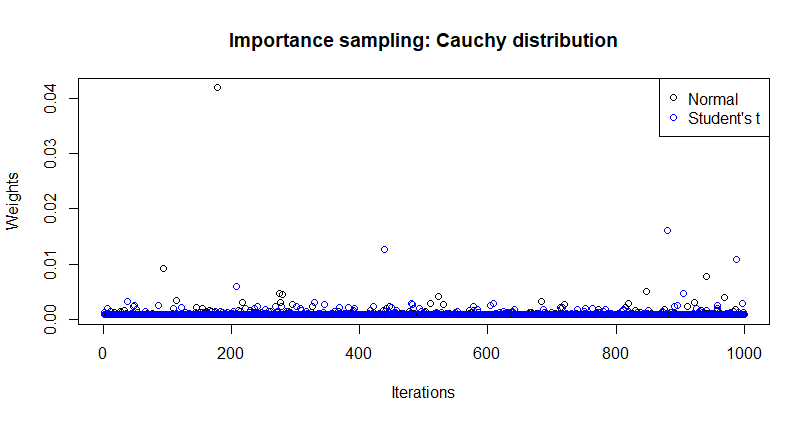
\includegraphics[width=340pt, height=200pt]{Chapters/chapter5/figures/ISexampleCauchy.png}
	%%\centerline{\epsfig{/Chapters/chapter1/figures/cat.eps,width=.8\textheight,height=.4\textwidth}}
	\caption[List of figure caption goes here]{Importance sampling: 1000 draws of a Cauchy distribution using the standard normal and student's t with 3 degrees of freedom as proposals.}\label{fig55}
\end{figure} 

\begin{figure}[!h]
	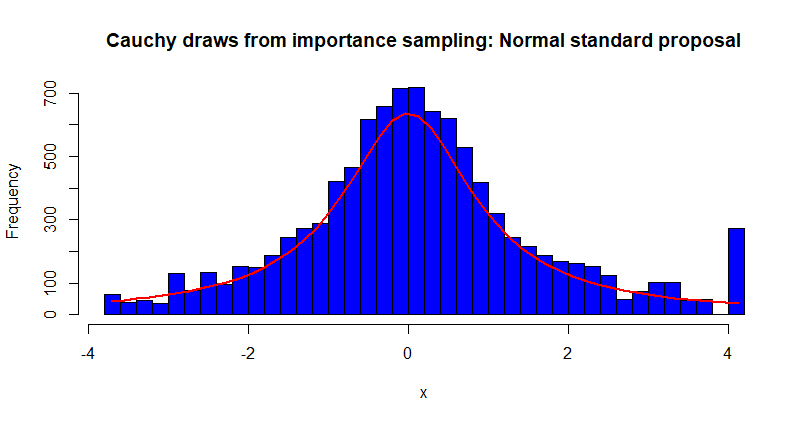
\includegraphics[width=340pt, height=200pt]{Chapters/chapter5/figures/IScauchyNormal.png}
	%%\centerline{\epsfig{/Chapters/chapter1/figures/cat.eps,width=.8\textheight,height=.4\textwidth}}
	\caption[List of figure caption goes here]{Importance sampling: Draws from a Cauchy distribution using the standard normal as proposal.}\label{fig56}
\end{figure} 

\begin{figure}[!h]
	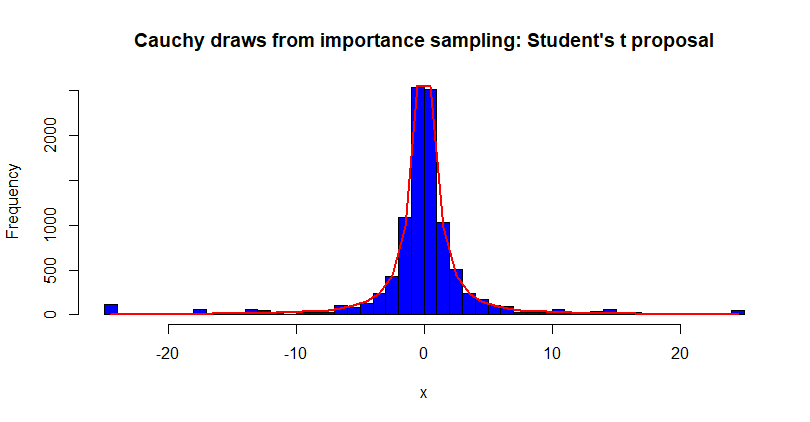
\includegraphics[width=340pt, height=200pt]{Chapters/chapter5/figures/IScauchyStudent.png}
	%%\centerline{\epsfig{/Chapters/chapter1/figures/cat.eps,width=.8\textheight,height=.4\textwidth}}
	\caption[List of figure caption goes here]{Importance sampling: Draws of a Cauchy distribution using the Student's t with 3 degrees of freedom as proposal.}\label{fig57}
\end{figure}       

\section{Particle filtering}\label{sec53}

Now, we consider the scenario where we need to sample from a posterior distribution whose dimension increases over time, $\pi(\bm{\theta}_{0:t}|\bm{y}_{0:t})$, for $t = 0, 1, \dots$. The challenge arises from the fact that, even if this posterior distribution is known, the computational complexity of implementing a sampling scheme in this context increases linearly with $t$. This makes MCMC methods, which operate in batch mode and require a complete re-run whenever new information becomes available, less optimal. Consequently, we present sequential algorithms, which operate incrementally as new data becomes available, and are often a better alternative. These algorithms are typically faster and are well-suited for scenarios requiring real-time updates, commonly referred to as online mode.

Specifically, we consider the dynamic system in the \textit{state-space} representation. This is a system where there is an \textit{unobservable state vector} $\bm{\theta}_t\in\mathbb{R}^K$, and an observed variable $\bm{Y}_t$, $t=0,1,\dots$ such that (i) $\bm{\theta}_t$ is a \textit{Markov process}, this is, $\pi(\bm{\theta}_{t}|\bm{\theta}_{1:t-1})=\pi(\bm{\theta}_{t}|\bm{\theta}_{t-1})$, $t=1,2,\dots$, all the relevant information to define $\bm{\theta}_{t}$ is in $\bm{\theta}_{t-1}$,\footnote{$\bm{\theta}_{0}$ comes from the given distribution $\pi(\bm{\theta}_{0})$.} and ii) $\bm{Y}_t\perp \bm{Y}_s|\bm{\theta}_{t}$, $s<t$, there is independence between observable variables regarding their history conditional on the actual state vector. We can see in Figure \ref{fig:state_space} a graphical representation of the dynamic system.
\begin{figure}[h!]
\centering
%\resizebox{1\textwidth}{!}{%
%	\begin{threeparttable}
%		\includegraphics[width = \linewidth, page = 1]
\begin{tikzpicture}[
	every node/.style={font=\small},
	obs/.style={rectangle, draw=black, fill=gray!20, minimum size=12mm},
	state/.style={circle, draw=black, fill=gray!20, minimum size=12mm},
	arrow/.style={-Latex, thick},
	node distance=1.5cm and 2.5cm
	]
	
	% Nodes
	\node[state] (x_t-1) {$\bm{\theta}_{t-1}$};
	\node[state, right=of x_t-1] (x_t) {$\bm{\theta}_{t}$};
	\node[state, right=of x_t] (x_t+1) {$\bm{\theta}_{t+1}$};
	
	\node[obs, above=of x_t-1] (y_t-1) {$Y_{t-1}$};
	\node[obs, above=of x_t] (y_t) {$Y_t$};
	\node[obs, above=of x_t+1] (y_t+1) {$Y_{t+1}$};
	
	% Arrows
	\draw[arrow] (x_t-1) -- (x_t);
	\draw[arrow] (x_t) -- (x_t+1);
	
	\draw[arrow] (x_t-1) -- (y_t-1);
	\draw[arrow] (x_t) -- (y_t);
	\draw[arrow] (x_t+1) -- (y_t+1);
	
	% Text
	\node[align=center, below=0.5cm of x_t] (text1) {$\bm{\theta}_{t} \sim \pi(\bm{\theta}_{t} | \bm{\theta}_{t-1})$};
	\node[align=center, above=0.5cm of y_t] (text2) {$Y_t \sim p(Y_t | \bm{\theta}_{t})$};
%\node[align=center, below=2.5cm of x_t, font=\small] (note) 
%{};
\end{tikzpicture}
%\end{threeparttable}%
%}
\begin{tablenotes}
	\item \small{\textbf{Notes:} The figure illustrates the structure of a \textit{state-space} model where the latent states $\bm{\theta}_t$ evolve according to $\pi(\bm{\theta}_t | \bm{\theta}_{t-1})$, and the observations $Y_t$ depend on the states via $p(Y_t | \bm{\theta})$.}
\end{tablenotes}
\caption{\textit{State-space} model representation.}
\label{fig:state_space}
\end{figure}

Formally,
\begin{align*}
	\bm{\theta}_t &= h(\bm{\theta}_{t-1}, \bm{w}_t) & \text{(State equations)}\nonumber\\
	Y_t & = f(\bm{\theta}_t, \mu_t)& \text{(Observation equation)},
\end{align*}
where $\bm{w}_t$ and $\mu_t$ are stochastic errors such that their probability distributions define the transition density $\pi(\bm{\theta}_t|\bm{\theta}_{t-1})$ and observation density $p(Y_t|\bm{\theta}_t)$. 

We present \textit{particle filtering}, a specific case of \textit{sequential Monte Carlo} (SMC), which is one of the most commonly used algorithms for scenarios requiring sequential updates of the posterior distribution as described by the \textit{state-space} model.

The starting point is \textit{sequential importance sampling} (SIS), originally proposed by \cite{handschin1969monte}, which is a modification of IS to compute an estimate of $\pi(\bm{\theta}_{0:t}|\bm{y}_{0:t})$ without altering the past trajectories $\left\{\bm{\theta}^{(s)}_{1:t-1}, s=1,2,\dots,S\right\}$. The key idea is to use a proposal density that takes the form

\begin{align*}
	q(\bm{\theta}_{0:t}|\bm{y}_{0:t}) &= q(\bm{\theta}_{0:t-1}|\bm{y}_{1:t-1})q(\bm{\theta}_t|\bm{\theta}_{t-1},\bm{y}_{t}) \\
	&= q(\bm{\theta}_0)\prod_{h=1}^{t}q(\bm{\theta}_h|\bm{\theta}_{h-1},\bm{y}_{h}).
\end{align*}

This proposal density allows calculating the weights sequentially,
\begin{align*}
	w_{t}(\bm{\theta}^{(s)}_{0:t})&=\frac{\pi(\bm{\theta}_{0:t}^{(s)}|\bm{y}_{0:t})}{q(\bm{\theta}_{0:t}^{(s)}|\bm{y}_{0:t})}\\
	&=\frac{p(\bm{y}_{0:t}|\bm{\theta}_{0:t}^{(s)})\pi(\bm{\theta}_{0:t}^{(s)})}{p(\bm{y}_{0:t})q(\bm{\theta}_{0:t}^{(s)}|\bm{y}_{0:t})}\\
	&=\frac{p(\bm{y}_{t}|\bm{\theta}_{t}^{(s)})p(\bm{y}_{1:t-1}|\bm{\theta}_{0:t-1}^{(s)})\pi(\bm{\theta}_{t}^{(s)}|\bm{\theta}_{t-1}^{(s)})\pi(\bm{\theta}_{0:t-1}^{(s)})}{p(\bm{y}_{0:t})q(\bm{\theta}_{t}^{(s)}|\bm{\theta}_{t-1}^{(s)},\bm{y}_{t})q(\bm{\theta}_{0:t-1}^{(s)}|\bm{y}_{1:t-1})}\\
	&\propto\frac{p(\bm{y}_{1:t-1}|\bm{\theta}_{0:t-1}^{(s)})\pi(\bm{\theta}_{0:t-1}^{(s)})}{q(\bm{\theta}_{0:t-1}^{(s)}|\bm{y}_{1:t-1})}\frac{p(\bm{y}_{t}|\bm{\theta}_{t}^{(s)})\pi(\bm{\theta}_{t}^{(s)}|\bm{\theta}_{t-1}^{(s)})}{q(\bm{\theta}_{t}^{(s)}|\bm{\theta}_{t-1},\bm{y}_{t}^{(s)})}\\
	&\propto w_{t-1}(\bm{\theta}^{(s)})\frac{p(\bm{y}_{t}|\bm{\theta}_{t}^{(s)})\pi(\bm{\theta}_{t}|\bm{\theta}_{t-1}^{(s)})}{q(\bm{\theta}_t^{(s)}|\bm{\theta}_{t-1}^{(s)},\bm{y}_{t})}\\
	&\propto w_{t-1}^*(\bm{\theta}^{(s)})\frac{p(\bm{y}_{t}|\bm{\theta}_{t}^{(s)})\pi(\bm{\theta}_{t}|\bm{\theta}_{t-1}^{(s)})}{q(\bm{\theta}_t^{(s)}|\bm{\theta}_{t-1}^{(s)},\bm{y}_{t})}.
\end{align*} 
Take into account that $p(\bm{y}_{0:t})$ does not depend on $\bm{\theta}^{(s)}_{0:t}$. The term $\alpha_t(\bm{\theta}_{0:t}^{(s)})=\frac{p(\bm{y}_{t}|\bm{\theta}_{t}^{(s)})\pi(\bm{\theta}_{t}|\bm{\theta}_{t-1}^{(s)})}{q(\bm{\theta}_t^{(s)}|\bm{\theta}_{t-1}^{(s)},\bm{y}_{t})}$ is called the \textit{incremental importance weight}, and implies that
$$w_t(\bm{\theta}^{s}_{0:t})=w_0(\bm{\theta}^{s}_{0})\prod_{h=1}^{t}\alpha_h(\bm{\theta}_{1:h}^{(s)}).$$ 

This algorithm possesses the desirable property of maintaining fixed computational complexity. Consequently, we sequentially obtain draws $\bm{\theta}_t^{(s)}$, referred to as particles: $\bm{\theta}_0^{(s)}$ is drawn from $q(\bm{\theta}_0)$ at $t=0$, and subsequently, $\bm{\theta}_h^{(s)}$ is drawn from $q(\bm{\theta}_h|\bm{\theta}_{h-1},\bm{y}_{h})$ at $t=h$ \cite{doucet2001introduction,cappe2007overview}.

A relevant case is when the proposal distribution takes the form of the prior distribution, that is, $q(\bm{\theta}_{0:t}|\bm{y}_{0:t}) = \pi(\bm{\theta}_{0:t}) = \pi(\bm{\theta}_0)\prod_{h=1}^{t}\pi(\bm{\theta}_h|\bm{\theta}_{h-1})$. This implies that
\begin{align*}
	w_{t}(\bm{\theta}^{(s)})&\propto w_{t-1}^*(\bm{\theta}^{(s)})p(\bm{y}_{t}|\bm{\theta}_{t}^{(s)}),
\end{align*}
this means that the \textit{incremental importance weight} is given by $p(\bm{y}_{t}|\bm{\theta}_{t}^{(s)})$. 

Algorithm \ref{Alg:SIS} shows how to perform SIS \cite{cappe2007overview}. We set $w_t^{(s)}:=w_t(\bm{\theta}_{0:t}^{(s)}$ to simplify notation.\\
\begin{algorithm}[h!]
	\caption{Sequential importance sampling algorithm}\label{Alg:SIS}
	\begin{algorithmic}[1]
		\For{\texttt{$s=1,\dots,S$}}
		\State Sample $\bm{\theta}_0^{(s)}$ from $q(\bm{\theta}_0|y_0)$
		\State Calculate the importance weights $w_0^{(s)}\propto\frac{p(y_0|\bm{\theta}_0^{(s)})\pi(\bm{\theta}_0^{(s)})}{q(\bm{\theta}_0^{(s)}|y_0)}$ 
		\EndFor 
		\For{\texttt{$t=1,\dots,T$}}  		 			
			\For{\texttt{$s=1,\dots,S$}}
				\State Draw particles $\bm{\theta}_t^{(s)}$ from $q_t(\bm{\theta}_t|\bm{\theta}_{t-1}, \bm{y}_t)$
				\State Compute the weights $w_t^{(s)}=w_{t-1}^{*(s)}\frac{p(\bm{y}_{t}|\bm{\theta}_{t}^{(s)})\pi(\bm{\theta}_{t}^{(s)}|\bm{\theta}_{t-1}^{(s)})}{q(\bm{\theta}_t^{(s)}|\bm{\theta}_{t-1}^{(s)},\bm{y}_{t})}$
			\EndFor
			\State Standardize the weights $w_t^{*(s)}=\frac{w_t^{(s)}}{\sum_{h=1}^Sw_t^{(h)}}$, $s=1,2,\dots,S$  
		\EndFor
	\end{algorithmic} 
\end{algorithm}

\textbf{Example: Dynamic linear model}

Let's assume that the state-space representation is  
\begin{align*}
	{\theta}_t &= {\theta}_{t-1} + {w}_t & \text{(State equation)} \nonumber\\
	Y_t & = \phi {\theta}_t + \mu_t & \text{(Observation equation)},
\end{align*}
where ${w}_t\sim N(0, \sigma_w^2)$ and $\mu_t\sim N(0,\sigma_{\mu}^2)$, $t=1,2,\dots,50$. In addition, we use the proposal distribution $q(\theta_t|y_t)=\pi(\theta_t)$, which is normal with mean $\theta_{t-1}$ and variance $\sigma_w^2$. Then, the weights are given by the recursion  
\[ 
w_t^{(s)} \propto w_{t-1}^{*(s)} p(y_t|\theta_t,\sigma_{\mu}^2), 
\]  
where $p(y_t|\theta_t,\sigma_{\mu}^2)$ is $N(\phi \theta_t, \sigma_{\mu}^2)$.  

We can compute the mean and standard deviation of the state at each $t$ using  
\[
\hat{\theta}_t = \sum_{s=1}^S w_t^{*(s)} \theta_t^{(s)}
\]  
and  
\[
\hat{\sigma}_{\theta} = \left(\sum_{s=1}^S w_t^{*(s)} \theta_t^{2(s)} - \hat{\theta}_t^2\right)^{1/2}.
\]  

The following code demonstrates the implementation of this algorithm, setting $\sigma_w^2=\sigma_{\mu}^2=1$ and $\phi=0.5$. First, we simulate the process, and then we implement the SIS algorithm.

\begin{tcolorbox}[enhanced,width=4.67in,center upper,
	fontupper=\large\bfseries,drop shadow southwest,sharp corners]
	\textit{R code. Sequential importance sampling: Dynamic linear model}
	\begin{VF}
		\begin{lstlisting}[language=R]
rm(list = ls()); set.seed(010101)
S <- 50000 # Number of particles
sigma_w <- 1  # State noise
sigma_mu <- 1  # Observation noise
phi <- 0.5 # Coefficient in observation equation
T <- 50 # Sample size
# Simulate true states and observations
theta_true <- numeric(T); y_obs <- numeric(T)
theta_true[1] <- rnorm(1, mean = 0, sd = sigma_w)  # Initial state
for (t in 2:T) {
	theta_true[t] <- rnorm(1, mean = theta_true[t-1], sd = sigma_w)
}
y_obs <- rnorm(T, mean = phi*theta_true, sd = sigma_mu)
# Sequential Importance Sampling (SIS)
particles <- matrix(0, nrow = S, ncol = T) 
weights <- matrix(0, nrow = S, ncol = T) 
weightsSt <- matrix(0, nrow = S, ncol = T) 
# Initialization
particles[, 1] <- rnorm(S, mean = 0, sd = sigma_w)  # Sample initial particles
weights[, 1] <- dnorm(y_obs[1], mean = phi*particles[, 1], sd = sigma_mu)  # Importance weights
weightsSt[, 1] <- weights[, 1] / sum(weights[, 1])  # Standardized weights
# Sequential updating
for (t in 2:T) {
	# Propagate particles
	particles[, t] <- rnorm(S, mean = particles[, t-1], sd = sigma_w)
	# Compute weights
	weights[, t] <- weightsSt[, t-1] * dnorm(y_obs[t], mean = phi*particles[, t], sd = sigma_mu) # Recursive weight update
	weightsSt[, t] <- weights[, t] / sum(weights[, t])  # Normalize weights
}
# Estimate the states (weighted mean)
FilterDist <- colSums(particles * weightsSt)
SDFilterDist <- (colSums(particles^2 * weightsSt) - FilterDist^2)^0.5
library(dplyr); library(ggplot2); library(latex2exp)
ggplot2::theme_set(theme_bw())
df <- tibble(t = 1:T, mean = FilterDist, lower = FilterDist - 2*SDFilterDist, upper = FilterDist + 2*SDFilterDist, theta_true = theta_true)
# Function to plot
plot_filtering_estimates <- function(df) {
	p <- ggplot(data = df, aes(x = t)) + geom_ribbon(aes(ymin = lower, ymax = upper), alpha = 1, fill = "lightblue") + geom_line(aes(y = theta_true), colour = "black", alpha = 1, linewidth = 0.5) + geom_line(aes(y = mean), colour = "blue", linewidth = 0.5) + ylab(TeX("$\\theta_{t}$")) + xlab("Time")
	print(p)
}
plot_filtering_estimates(df)
\end{lstlisting}
	\end{VF}
\end{tcolorbox} 

Figure \ref{fig58} shows the trajectory of the true state vector (black line), the posterior mean (blue line), and the area defined by $\pm2\hat{\sigma}_{\theta}$ (light blue shaded area).

\begin{figure}[!h]
	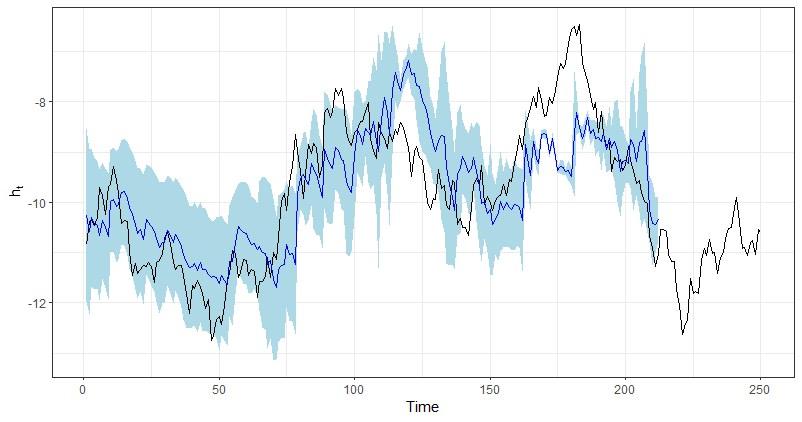
\includegraphics[width=340pt, height=200pt]{Chapters/chapter5/figures/SIS.png}
	\caption[List of figure caption goes here]{State in linear state-space model: True and mean estimate using sequential importance sampling, $T=50$.}\label{fig58}
\end{figure} 

Sequential importance sampling is effective for sampling from the posterior distribution in the short term. However, it is important to note that SIS is a particular case of IS and, consequently, inherits the drawbacks of importance sampling. In particular, the variance of the weights increases exponentially with $t$ \cite{kong1994sequential}. This implies that, as $t$ increases, the importance weights tend to degenerate in the long run; that is, all probability mass concentrates on a few weights, a phenomenon known as sample impoverishment or weight degeneracy. This is because is impossible to accurately
represent a distribution on a space of arbitrarily high dimension with a sample of fixed, finite size. This phenomenon can be observed, for instance, in the dynamic linear model example, where the highest standardized weight at $t=50$ is 53\%, and 7 out of 50,000 particles account for 87\% of the total probability.

Given that, in practice, we are often interested in lower-dimensional marginal distributions, ideas from sampling/importance resampling can be employed. This strategy avoids the accumulation of errors due to resetting the system, although resampling introduces some additional Monte Carlo variation. \cite{Gordon1993} proposed the \textit{Bootstrap filter}, where, at each time step, resampling is performed by drawing $S$ particles from the current set using the standardized weights as probabilities of selection. This ensures that particles with small weights have a low probability of being selected. After resampling, the standardized weights are set equal to $1/S$. Note that the \textit{Bootstrap filter} involves multiple iterations of the SIR algorithm, which implies that the resampled trajectories are no longer independent. This multinomial resampling provides an unbiased approximation to the posterior distribution obtained by SIS \cite{doucet2009tutorial}. Additionally, other resampling approaches preserve the unbiasedness property while offering a reduction in variance, such as residual resampling \cite{Liu1995} and systematic resampling \cite{Carpenter1999}. 

Algorithm \ref{Alg:PF} shows how to perform the \textit{particle filter}. We set $w_t^{(s)}:=w_t(\bm{\theta}_{0:t}^{(s)}$ to simplify notation. \cite{doucet2009tutorial}.\\
\begin{algorithm}[h!]
	\caption{The \textit{particle filter} algorithm}\label{Alg:PF}
	\begin{algorithmic}[1]
		\For{\texttt{$s=1,\dots,S$}}
		\State Sample $\bm{\theta}_0^{(s)}$ from $q(\bm{\theta}_0|y_0)$
		\State Calculate the importance weights $w_0^{(s)}\propto\frac{p(y_0|\bm{\theta}_0^{(s)})\pi(\bm{\theta}_0^{(s)})}{q(\bm{\theta}_0^{(s)}|y_0)}$
		\EndFor
		\State Standardize the weights $w_0^{*(s)}=\frac{w_0^{(s)}}{\sum_{h=1}^Sw_0^{(h)}}$, $s=1,2,\dots,S$
		\State Select $S$ particles from $\left\{\bm{\theta}_0^{(s)},w_0^{*(s)}\right\}$ to obtain $\left\{\bm{\theta}_0^{r(s)},1/S\right\}$  
		\For{\texttt{$t=1,\dots,T$}}  		 			
		\For{\texttt{$s=1,\dots,S$}}
		\State Draw particles $\bm{\theta}_t^{(s)}$ from $q_t(\bm{\theta}_t|\bm{\theta}_{t-1}, \bm{y}_t)$
		\State Set $\bm{\theta}_{1:t}^{(s)}\leftarrow (\bm{\theta}_{t-1}^{r(s)},\bm{\theta}_{t}^{(s)})$ 
		\State Compute the weights $\alpha_t^{(s)}=\frac{p(\bm{y}_{t}|\bm{\theta}_{t}^{(s)})\pi(\bm{\theta}_{t}^{(s)}|\bm{\theta}_{t-1}^{(s)})}{q(\bm{\theta}_t^{(s)}|\bm{\theta}_{t-1}^{(s)},\bm{y}_{t})}$		
		\EndFor
		\State Standardize the weights $w_t^{*(s)}=\frac{w_t^{(s)}}{\sum_{h=1}^Sw_t^{(h)}}$, $s=1,2,\dots,S$ 
		\State Select $S$ particles from $\left\{\bm{\theta}_{1:t}^{(s)},w_t^{*(s)}\right\}$ to obtain $\left\{\bm{\theta}_{1:t}^{r(s)},1/S\right\}$  
		\EndFor
	\end{algorithmic} 
\end{algorithm}

\textbf{Example: Dynamic linear model continues}

Let's apply the SIS algorithm to the dynamic linear model with a sample size of 200. Figure \ref{fig59} illustrates the performance of sequential importance sampling. We observe that the algorithm's performance deteriorates as $t$ increases. This is due to particle degeneration; at $t=200$, a single particle holds a weight close to 100\%.

\begin{figure}[!h]
	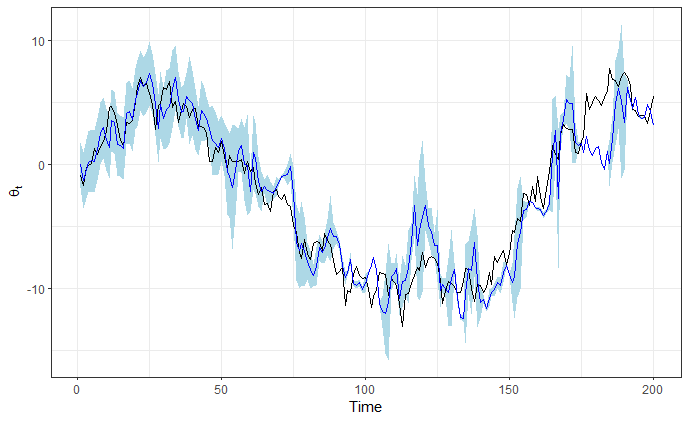
\includegraphics[width=340pt, height=200pt]{Chapters/chapter5/figures/SIS200.png}
	\caption[List of figure caption goes here]{State in linear state-space model: True and mean estimate using sequential importance sampling, $T=200$.}\label{fig59}
\end{figure} 

Let's perform particle filtering in this example. The following code illustrate the procedure.

Figure \ref{fig510} show the performance of particle filtering in this example. There is the true state vector (black line), the means based on $\left\{\bm{\theta}_{1:t}^{(s)},w_t^{*(s)}\right\}$ (blue line) and  $\left\{\bm{\theta}_{1:t}^{r(s)},1/S\right\}$ (purple line), and the area defined by $\pm2\hat{\sigma}_{\theta}$ based on the former (light blue shaded area). Note that the particle filtering algorithm has better performance than the SIS algorithm.   

\begin{figure}[!h]
	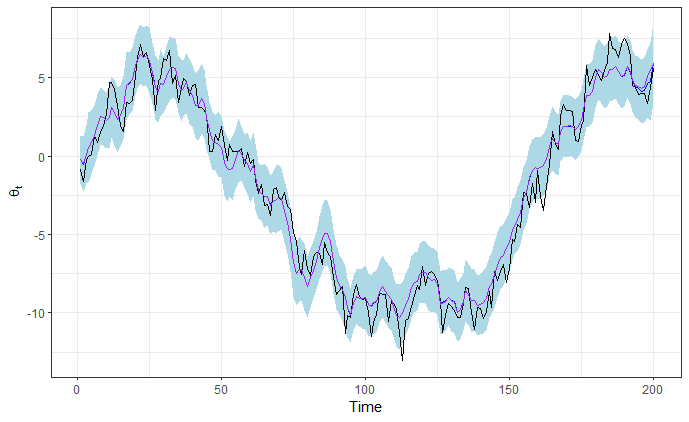
\includegraphics[width=340pt, height=200pt]{Chapters/chapter5/figures/PF.png}
	\caption[List of figure caption goes here]{State in linear state-space model: True and mean estimate using particle filtering, $T=200$.}\label{fig510}
\end{figure} 

\begin{tcolorbox}[enhanced,width=4.67in,center upper,
	fontupper=\large\bfseries,drop shadow southwest,sharp corners]
	\textit{R code. Particle filtering: Dynamic linear model}
	\begin{VF}
		\begin{lstlisting}[language=R]
rm(list = ls()); set.seed(010101)
S <- 50000 # Number of particles
sigma_w <- 1; sigma_mu <- 1  #  # State and observation noises
phi <- 0.5 # Coefficient in observation equation
T <- 200 # Sample size
# Simulate true states and observations
theta_true <- numeric(T); y_obs <- numeric(T)
theta_true[1] <- rnorm(1, mean = 0, sd = sigma_w) 
for (t in 2:T) {
	theta_true[t] <- rnorm(1, mean = theta_true[t-1], sd = sigma_w)
}
y_obs <- rnorm(T, mean = phi*theta_true, sd = sigma_mu)
# Particle filtering
particles <- matrix(0, nrow = S, ncol = T)  # Store particles
particlesT <- matrix(0, nrow = S, ncol = T)  # Store resampling particles
weights <- matrix(0, nrow = S, ncol = T)   # Store weights
weightsSt <- matrix(0, nrow = S, ncol = T)   # Store standardized weights
weightsSTT <- matrix(1/S, nrow = S, ncol = T)   # Store standardized weights
logalphas <- matrix(0, nrow = S, ncol = T)   # Store log incremental weights
particles[, 1] <- rnorm(S, mean = 0, sd = sigma_w) 
weights[, 1] <- dnorm(y_obs[1], mean = phi*particles[, 1], sd = sigma_mu)  # Importance weights
weightsSt[, 1] <- weights[, 1] / sum(weights[, 1])  # Normalize weights
ind <- sample(1:S, size = S, replace = TRUE, prob = weightsSt[, 1]) # Resample 
particles[, 1] <- particles[ind, 1] # Resampled particles
particlesT[, 1] <- particles[, 1] # Resampled particles
# Sequential updating
pb <- winProgressBar(title = "progress bar", min = 0, max = T, width = 300)
for (t in 2:T) {
	particles[, t] <- rnorm(S, mean = particles[, t-1], sd = sigma_w)
	logalphas[, t] <- dnorm(y_obs[t], mean = phi*particles[, t], sd = sigma_mu, log = TRUE) 
	weights[, t] <- exp(logalphas[, t])
	weightsSt[, t] <- weights[, t] / sum(weights[, t])
	if(t < T){
		ind <- sample(1:S, size = S, replace = TRUE, prob = weightsSt[, t])
		particles[, 1:t] <- particles[ind, 1:t]
	}else{
		ind <- sample(1:S, size = S, replace = TRUE, prob = weightsSt[, t])
		particlesT[, 1:t] <- particles[ind, 1:t]
	}
	setWinProgressBar(pb, t, title=paste( round(t/T*100, 0), "% done"))
}
close(pb)
\end{lstlisting}
	\end{VF}
\end{tcolorbox} 

\begin{tcolorbox}[enhanced,width=4.67in,center upper,
	fontupper=\large\bfseries,drop shadow southwest,sharp corners]
	\textit{R code. Particle filtering: Dynamic linear model}
	\begin{VF}
		\begin{lstlisting}[language=R]
FilterDist <- colSums(particles * weightsSt)
SDFilterDist <- (colSums(particles^2 * weightsSt) - FilterDist^2)^0.5
FilterDistT <- colSums(particlesT * weightsSTT)
SDFilterDistT <- (colSums(particlesT^2 * weightsSTT) - FilterDistT^2)^0.5
MargLik <- colMeans(weights)
plot(MargLik, type = "l")
library(dplyr)
library(ggplot2)
require(latex2exp)
ggplot2::theme_set(theme_bw())
df <- tibble(t = 1:T, mean = FilterDist, lower = FilterDist - 2*SDFilterDist, upper = FilterDist+ 2*SDFilterDist, meanT = FilterDistT, lowerT = FilterDistT - 2*SDFilterDistT,
upperT = FilterDistT + 2*SDFilterDistT, x_true = theta_true)
plot_filtering_estimates <- function(df) {
	p <- ggplot(data = df, aes(x = t)) + geom_ribbon(aes(ymin = lower, ymax = upper), alpha = 1, fill = "lightblue") + geom_line(aes(y = x_true), colour = "black", alpha = 1, linewidth = 0.5) + geom_line(aes(y = mean), colour = "blue", linewidth = 0.5) +
	geom_line(aes(y = meanT), colour = "purple", linewidth = 0.5) + 	ylab(TeX("$\\theta_{t}$")) + xlab("Time")
	print(p)
}
plot_filtering_estimates(df)
\end{lstlisting}
	\end{VF}
\end{tcolorbox} 

Algorithm \ref{Alg:PF} performs resampling at every time step. However, it is common to perform resampling only when the effective sample size of the particles ($ESS = (\sum_{s=1}^S (w_t^{*(s)})^{2})^{-1}$) falls below a specific threshold, such as 50\% of the initial number of particles. Note that when $w_t^{*(s)} = 1/S$, the effective sample size is equal to $S$, the total number of particles. Additionally, we should use $\left\{\bm{\theta}_{1:t}^{(s)},w_t^{*(s)}\right\}$ to estimate the posterior distribution, as it results in lower Monte Carlo error compared to calculations based on $\left\{\bm{\theta}_{1:t}^{r(s)},1/S\right\}$ \cite{cappe2007overview}. Finally, an estimate of the marginal likelihood can be obtained using $\hat{p}(y_t) = \frac{1}{S}\sum_{s=1}^S w_t^{(s)}$.

\textit{Particle filtering} has good advantages such as It is very quick and easy to implement, It is modular, that is, when changing the problem one need only change the expressions for the importance distribution and the importance weights, It can be straightforwardly implemented on a parallel algorithm. Allows easily carrying out sequential inference for very complex models. However, it also suffers from The resampling step introduces extra MC variability. The use of the state transition density as importance distribution can often lead to poor performance, which is manifested in a lack of robustness with respect to the values taken by the observed sequence, for example when outliers occur in the data or on the contrary when the variance of the observation noise is small. This procedure is not well suited to sample from $\pi(\bm{\theta}_{0:t}|y_{1:t})$. This is because most of the particles come from the same ancestor.



 

\section{Convergence diagnostics}\label{sec54}

\subsection{Numerical standard error}
\subsection{Effective sample size}
\subsection{Checking for errors in the posterior simulator}

\cite{geweke2004getting}

\subsection{Tests of convergence}

Regarding convergence issues, we implement several diagnostics to assess the adequacy of the posterior chains \cite{Plummer2016} in our Graphical User Interface (GUI). In particular, we should see that trace plots should appear stable, and autocorrelation plots should decrease rapidly. 

Additionally, we apply Geweke's test \cite{Geweke1992}, which is a simple two-sample test of means. If the mean of the first window (10\% of the chain) is not significantly different from the mean of the second window (50\% of the chain), we conclude that the target distribution has converged.

The Raftery and Lewis test \cite{Raftery1992} is designed to calculate the approximate number of iterations ($S$), burn-in ($b$), and thinning parameter ($d$) required to estimate $p\left[H(\bm{\theta}) \leq h\right]$, where $H(\bm{\theta}): \mathcal{R}^k \rightarrow \mathcal{R}$, given a specific quantile of interest ($q$), precision ($r$), and probability ($p$). Their diagnostic is based on the dependence factor, $I = \frac{S + b}{S_{\text{Min}}}$, where $S_{\text{Min}} = \Phi^{-1}\left(\frac{1}{2}(p+1)\right)^2 q(1-q) / r^2$ and $\Phi(\cdot)$ is the standard normal cumulative distribution function. Values of $I$ much greater than 5 indicate a high level of dependence.

Heidelberger and Welch's test \cite{Heidelberger1983} uses a Cramér-von Mises statistic to test the null hypothesis that the sampled values, $\bm{\theta}^{(s)}$, are drawn from a stationary distribution. The statistic is given by $\text{CVM}(B_S) = \int_0^1 B_S(t)^2 dt$, where $B_S(t) = \frac{S_{\left[St\right]} - \left[St\right] \bar{\bm{\theta}}^S}{\sqrt{S p(0)}}$, $S_S = \sum_{s=1}^S \bm{\theta}^{(s)}$, $\bar{\bm{\theta}}^S = S_S / S$, and $p(0)$ is the spectral density at 0, with $0 \leq t \leq 1$. Under the null hypothesis, $B_S(t)$ converges in distribution to the Brownian bridge. 

This test is recursively applied until either the null hypothesis is not rejected, or $t = 50\%$ of the chain has been discarded. Subsequently, the half-width test calculates a 95\% confidence interval for the mean using the portion of the chain that passed the stationarity test. If the ratio of the half-width of this interval to the mean is less than 0.1, the test is considered passed.\\


\section{Summary}\label{sec55}


\section{Exercises}\label{sec56}

\begin{enumerate}
	\item \textbf{Example: The normal model with independent priors}
	
	Let's recap the math test exercise in Chapter \ref{chap4}, this time assuming independent priors. Specifically, let $Y_i \sim N(\mu, \sigma^2)$, where $\mu \sim N(\mu_0, \sigma_0^2)$ and $\sigma^2 \sim IG(\alpha_0 / 2, \delta_0 / 2)$. The sample size is 50, and the mean and standard deviation of the math scores are 102 and 10, respectively. We set $\mu_0 = 100$, $\sigma_0^2 = 100$, and $\alpha_0 = \delta_0 = 0.001$.
	
	\begin{itemize}
		\item Find the posterior distribution of $\mu$ and $\sigma^2$.
		\item Program a Gibbs sampler algorithm and plot the histogram of the posterior draws of $\mu$
	\end{itemize}

	\item Show that the Gibbs sampler is a particular case of the Metropolis-Hastings where the acceptance probability is equal to 1.
	
	\item Implement a Metropolis-Hastings to sample from the Cauchy distribution, $C(0,1)$, using as proposals a standard normal distribution and a Student's t distribution with 5 degrees of freedom.
	
	\item This exercise was proposed by Professor Hedibert Freitas Lopes, who cites \cite{thomas2021learning} as a useful reference for an introduction to Hamiltonian Monte Carlo in \textbf{R} and the \textit{hmclearn} package. The task is to obtain posterior draws using the Metropolis-Hastings and Hamiltonian Monte Carlo algorithms for the posterior distribution given by 
	\[
	\pi(\theta_1,\theta_2|\bm{y}) \propto \exp\left\{-\frac{1}{2}(\theta_1^2\theta_2^2 + \theta_1^2 + \theta_2^2 - 8\theta_1 - 8\theta_2)\right\}.
	\]
	
 \item \textbf{Ph.D. students sleeping hours continues}
\begin{enumerate}
	\item Use importance sampling based on a $U(0,1)$ proposal to obtain draws of $\bm{\theta}|\bm{y} \sim B(16.55,39.57)$ in the Ph.D. students' sleeping hours example in Chapter \ref{chap4}. Note that, based on Exercise 15 in Chapter \ref{chap4}, $\alpha_0 = 1.44$ and $\beta_0 = 2.57$.
	\item Compute the marginal likelihood in this context (Bernoulli-Beta model) and compare it to the result obtained using the Gelfand-Dey method.
\end{enumerate}
    
	
\end{enumerate}



